\begin{figure}
\centering
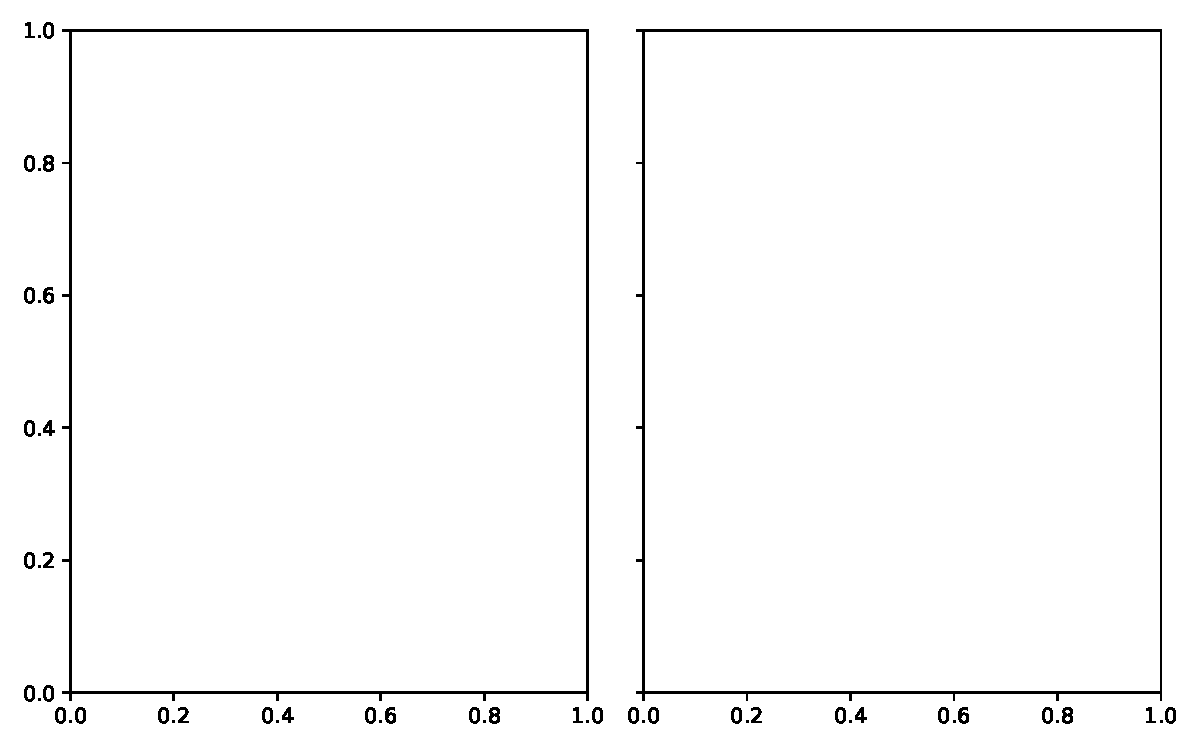
\includegraphics[width=\textwidth]{chapters/results/figures/comparison_intensity.pdf}
\caption{\label{fig:comparison-intensity}Distributions of total pixel intensities and
highest intensities in experimental and simulated decays. Top row compares experimental 
decays and all simulated decays. The bottom row shows the same distributions, but with simulated
decays split into single and double events. The calculations are done post normalization, so
the maximum possible intensity is 1.0.}
\end{figure}